\lesson{08/10}
\subsection{Braid Groups}
Consider a set of $n$ parallel, vertical strings: some operations can be done
to them, like undoing a passover of a string over another (Reidemeister move of the
second type) or putting the $i$'th string over the $i+1$'th, denoted by $\sigma_i$.
\begin{multicols}{2}
\begin{figure}[H]
    \centering
    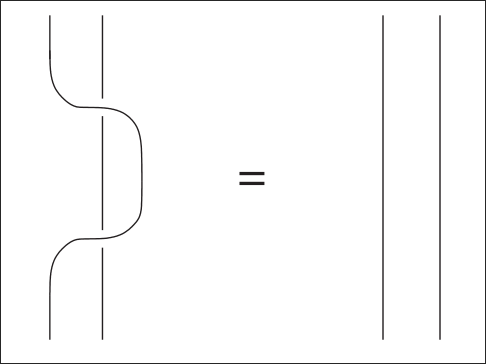
\includegraphics[width = .5\linewidth]{./Reidemeister.png}
    \caption{\small The Reidemeister move of the second type.}
\end{figure}
\begin{figure}[H]
    \centering
    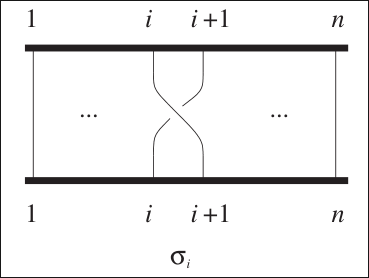
\includegraphics[width = .5\linewidth]{./sigma_1.png}
    \caption{\small The $\sigma_1$ operation.}
\end{figure}
\end{multicols}

A generic braid is a word
$$\sigma = \sigma_{j_1}^{i_1}...\sigma^{i_m}_{j_m}$$
with the generators $X_{n-1} = \left\{\sigma_1,\sigma_2,...,\sigma_{n-1}\right\}$.

To have meaningful braids, the strings must at least be $2$: a braid group with $n$
strings is denoted as $B_n$; the group $B_2$ is non-trivial:
$$B_2\cong(\mathbb{Z},+)$$

\textbf{Lemma} In the group $B_n$ with $n>2$,
$$\sigma_i\sigma_j=\sigma_j\sigma_i$$
if and only if $|i-j|\geq 2$.

This lemma is intuitively true, since the moves $\sigma_i,\sigma_j$ act on different
couples of strings if and only if $|i-j|\geq2$.

\textbf{Theorem} In the group $B_n$ with $n>2$,
$$\sigma_i\sigma_{i+1}\sigma_i = \sigma_{i+1}\sigma_i\sigma_{i+1} \forall i$$
This can be proven by executing the moves manually.

With these properties, the presentation of the group can be determined to be
$$B_n = \bra{\sigma_1,\sigma_2,...,\sigma_{n-1}}\ket{\sigma_i\sigma_j =
\sigma_j\sigma_i\,(|i-j|\geq2),\sigma_i\sigma_{i+1}\sigma_i =
\sigma_{i+1}\sigma_i\sigma_{i+1}\,(\forall i)}$$
\section{Continuous Groups}
\textbf{Def.} A group $G$ is said to be continuous if $G$ is infinite and
uncountable.

\textbf{Def.} A group $G$ is said to be discrete and continuous if $G$ is infinite
and countable, i.e. there exist a one-to-one correspondence with the natural numbers
$\mathbb{N}$.

Continuous groups are not necessarily vector spaces, so to characterize their size
the term "dimension" is a slight abuse of notation:

\textbf{Def.} Given a continuous group $G$, its dimension $\dim(G)\in\mathbb{N}$
is the number of independent real parameters, called \textit{coordinates} needed
to parametrize its elements.

If the product of two elements of the group
$$g_3=g_1\cdot g_2$$
depends \textit{smoothly} on the coordinates of the two elements, the set of
coordinates form a differential manifold, called the \textit{group manifold}.

\textbf{Def.} A group $G$ with coordinates that form a group manifold is called a
\textbf{Lie Group}.
\subsection{Simplest Lie groups}
The simplest Lie groups have dimension $1$, like
$$(\mathbb{R},+)$$
in which the coordinate choice is trivial, and
$$U(1) := \left\{z\in\mathbb{C} \text{ s.t. }|z|=1\right\}$$
in which the coordinate is $\alpha=\arg(z)$.

These can be combined, respectively, in
$$(\mathbb{R},+)\times(\mathbb{R},+)\times... = (\mathbb{R}^n,+)$$
and
$$[U(1)]^n=U(1)\times U(1)...=\left\{(z_1,z_2,...,z_n)\text{ s.t. }|z_i|=1\,\forall
i\right\}$$
which is isomorphic to the $n-$torus.
\subsection{Matrix Groups}
An important class of Lie groups are matrix groups: besides the somewhat trivial
group
$$\left(\text{Mat}(n\times m,\mathbb{R}),+\right)$$
the interesting groups have matrix multiplication as the group product and for this
reason all these groups are sets of invertible $n\times n$ matrices.
\begin{enumerate}
    \item General linear transformations on $\mathbb{R}^n$
        $$GL(n,\mathbb{R}):=\left\{A\in\text{Mat}(n\times n,\mathbb{R})\text{ s.t. }
        \det(A)\neq 0\right\}:$$
        this group has dimension $n^2$, since the inequality $\det(A)\neq 0$ does not
        reduce the number of independent parameters; as stated before, all matrix
        groups with multiplication as group product are
        subgroups of $GL(n,\mathbb{R})$.
    \item Special linear transformations on $\mathbb{R}^n$
        $$SL(n,\mathbb{R}):=\left\{A\in\text{Mat}(n\times n)\text{ s.t. }\det(A)=1
        \right\}:$$
        this group has dimension $\dim(SL(n,\mathbb{R})) = n^2-1$, since its
        dimension as a vector space coincides with the dimension of the manifold.
    \item Orthogonal group
        $$O(n):=\left\{A\in\text{Mat}(n\times n,\mathbb{R})\text{ s.t. }A^T=A^{-1}
        \right\}:$$
        these transformation preserve the norm of vectors in $\mathbb{R}^n$ and 
        the orthogonality condition implies that $\dim(O(n)) = \flatfrac{n(n-1)}{2}$
        and that $\det(A)=\pm1$; the subgroup with positive determinant is
        a subgroup of both $SL(n,\mathbb{R})$ and $O(n)$ and it is called the
        \textit{special} orthogonal group.
    \item Special Orthogonal Group
        $$SO(n) :=\left\{A\in O(n)\text{ s.t. } \det(A)=1\right\}:$$
        this group has the same dimension of $O(n)$.
    \item Unitary group
        $$U(n):=\left\{A\in\text{Mat}(n\times n,\mathbb{C})\text{ s.t. }A^\dagger=
        A^{-1}\right\}:$$
        this is the complex equivalent of $O(n)$ and, similarly, preserves the
        complex norm of $\mathbb{C}^n$ and admits a subgroup with $\det(A)=1$; it has
        dimension $\dim(U(n))=2n^2-\flatfrac{2n(n-1)}{2} - n =n^2$.
    \item Special Unitary Group
        $$SU(n) :=\left\{A\in U(n)\text{ s.t. } \det(A)=1\right\}:$$
        this group has the same dimension of $U(n)$ and it is one of the most
        important groups for physics, since $SU(2)$ is pivotal for the description
        of spin and of the Lorentz group; it has dimension $\dim(SU(n))=n^2-1$, since
        the condition $\det(A)=1=e^{i\alpha}$ constrains a parameter.
    \item Symplectic group
        $$Sp(2n,\mathbb{R}):=\left\{A\in\text{Mat}(2n\times 2n,\mathbb{R})
        \text{ s.t. } A^T\Omega A = \Omega,\,\forall\Omega\text{ symplectic form}
        \right\}:$$
        $\Omega$ is the symplectic form that should be familiar from Hamiltonian
        mechanics
        $$\Omega = \begin{pmatrix}
            \mathbb{O}_n&\mathbb{I}_n\\
            -\mathbb{I}_n&\mathbb{O}_n
        \end{pmatrix}
        $$
        \textbf{Note} For $n=1$, $Sp(2,\mathbb{R})=SL(2,\mathbb{R})$
\end{enumerate}

There are "exceptional" Lie groups that were discovered after classifying all the Lie
Algebras of continuous groups: $G_2,F_4,E_6,E_7,E_8$; they have some applications in
String Theory.

\subsection{Action of Groups}
\textbf{Def. }Given a group $G$ and a non-empty set $X$, a \textit{left action} $L$
of $G$ on $X$ is the group homomorphism
\begin{align*}
    L:\,&G\rightarrow\text{Perm}(X)\\
      &g\rightarrow L_g.
\end{align*}
If $L$ exists, $X$ is called a left $G$-space.

Since $L$ is a group homomorphism, it follows that
$$L_{g_1\cdot g_2} = L_{g_1}\circ L_{g_2}$$

\textbf{Def.} Given a group $G$ and a non-empty set $X$, a \textit{right action} $R$
of $G$ on $X$ is a function
$$\begin{aligned}
      R:\,&G\rightarrow\text{Perm}(X)\\
          &g\rightarrow R_g
  \end{aligned}\text{  so that } R_{g_1\cdot g_2} = R_{g_2}\circ R_{g_1}.
$$
If $R$ exists, $X$ is called a right $G$-space.

\textbf{Note} It can be shown that, if both $L,R$ exist, they are
isomorphic\footnote{?? How can there be an isomorphism between functions ??}.

\textbf{Def.} Given a left $G$-group $X$, an \textit{orbit} of an element $x\in X$ is
the set
$$O_x:=\left\{x'\in X\text{ s.t. }\exists g\in G \text{ s.t. }x' = L_g(x)\right\}.$$
\textbf{Example} Given $x\in X=\mathbb{R}^2$ and $G=SO(2)$, its orbit is the set
$$O_x = \left\{x'\in\mathbb{R}^2\text{ s.t. }|x'| = |x|\right\}$$
since for all points $x'\in\mathbb{R}^2=X$ that have the same norm as $x$ there
exist a rotation, i.e. an element of $SO(2)=G$, that transforms $x$ into $x'$.
\newpage
\textbf{Theorem} Belonging to the same orbit is an equivalence relation on $X$:
\begin{enumerate}
    \item $x\in O_x$ for all $x\in X$ (reflexive);
    \item $x'\in O_x \leftrightarrow x\in O_{x'}$ (symmetric);
    \item $x'\in O_x\land x''\in O_{x'} \rightarrow x''\in O_x$ (transitive). 
\end{enumerate}
\textbf{Proof}
The first statement can be proven considering that
$L_e = \text{Id}\in\text{Perm}(X)$, thus $x\in O_x$.

The second statement can be proven considering $x'\in O_x$ implies $\exists g$ so
that $x' = L_g(x)$: the inverse of this action is
$\left(L_g\right)^{-1} = L_{g^{-1}}$ and
$$(L_{g})^{-1}(x') = (L_{g^{-1}}\circ L_g)(x) = x$$
thus $g^{-1}\in G$ is so that $x=L_{g^{-1}}(x')$ and so $x\in O_{x'}$.

The third statement can be similarly proven using the group product: $x'=L_{g_1}(x)$,
$x'' = L_{g_2}(x')$, so
$$x'' = (L_{g_2})^{-1}(x') = (L_{g_2^{-1}}\circ L_{g_1^{-1}})(x) = L_{g_2^{-1}\cdot
g_1^{-1}}(x):$$
this means that $g_2^{-1}\cdot g_1^{-1}=g'\in G$ is so that $L_{g'}(x'') = x$, which
means $x''\in O_x$.\qed

\textbf{Def.} Given a left action $L$, it is a \textit{transitive left action} if
$$\exists y\in X\text{ s.t. } x\in O_y\,\forall x\in X$$
or, in other words, the set $X$ consists of only one equivalence class with respect
to the equivalence relation defined above.

\textbf{Example} Consider $X = \mathbb{R}^2$, $G = (\mathbb{R}^2,+)$ and $L$ as
translations on the plane: the left action is transitive, since every point $x\in
\mathbb{R}^2$ can be "reached" from any other point with a translation.
